\section{QRコード}
自動車メーカーのデンソーに発明された.
汚れによる耐障害性が非常に高く,非対称なので,向きの検出も可能.
英数字で最大4296文字まで記録が可能

\begin{figure}[htbp]
    \begin{center}
        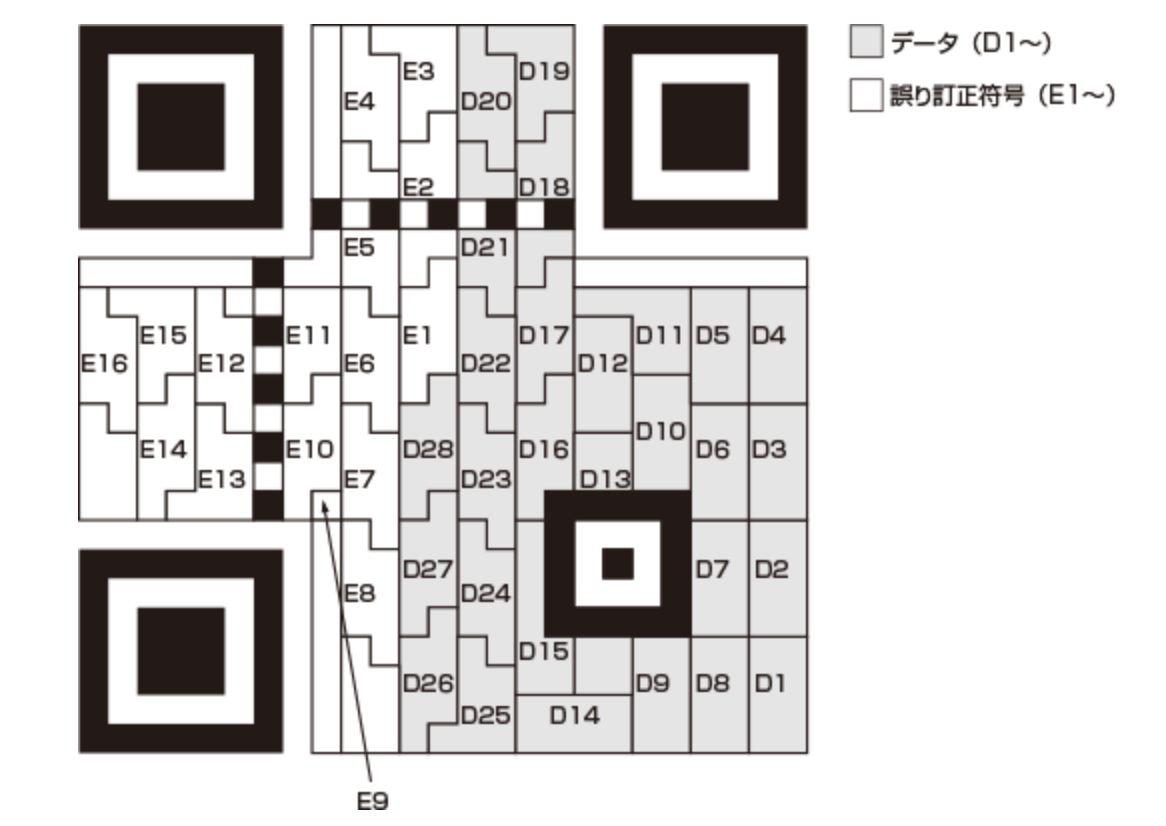
\includegraphics[clip,width=7.0cm]{img/qrcode.png}
        \caption{QRコードの仕様: https://ja.wikipedia.org/wiki/QR%E3%82%B3%E3%83%BC%E3%83%89}
    \end{center}
\end{figure}
